% 05-method.tex 中文版（中英对照用；不含 label，避免与英文版重复）
% file:line 落点指向 LINGSHU v5.1 参考实现。

\section{方法}

\begin{figure*}[t]
\centering
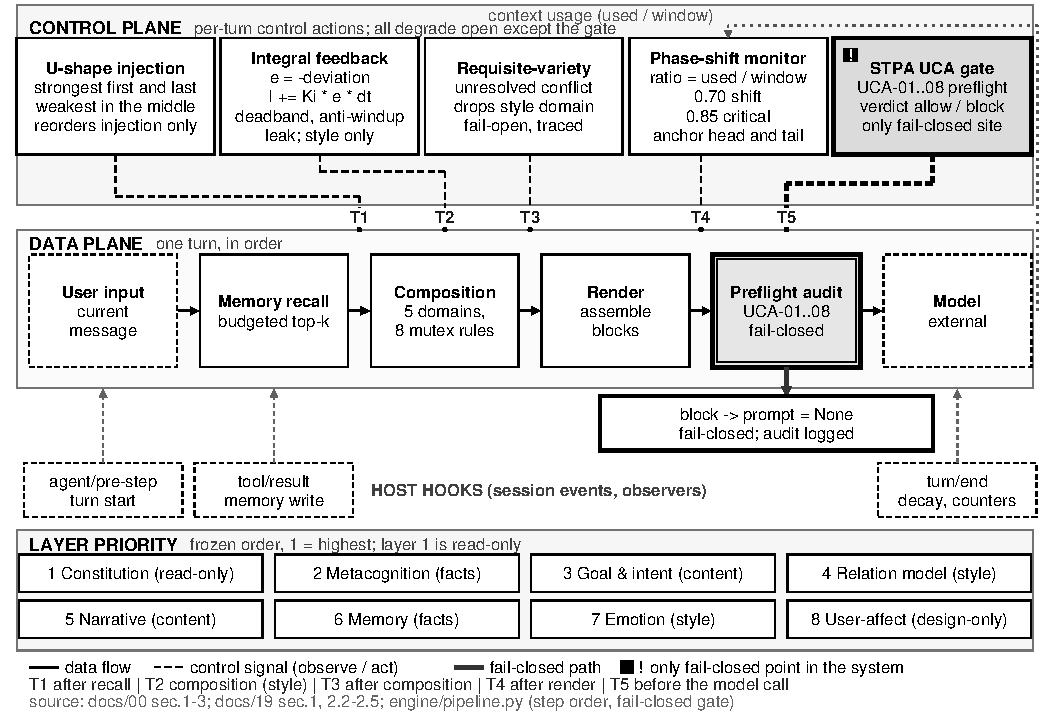
\includegraphics[width=0.98\textwidth]{figures/fig1-architecture.pdf}
\caption{控制面与数据面。数据面（下半部分）是每轮的注入路径：用户消息 $\rightarrow$
预算化召回 $\rightarrow$ 五域合成 $\rightarrow$ 渲染 $\rightarrow$ 前置审计 $\rightarrow$
外部模型。控制面（上半部分）观测上下文用量并对组装施加动作；STPA 闸门（阴影部分）是系统中
\emph{唯一}的 fail-closed 位置，因此一旦阻断就完全不返回可注入的 prompt。虚线是控制信号；
分层优先级条记录冻结的优先级（$1$ 最高，第 1 层只读）。来源：\texttt{docs/00} \S1--3、
\texttt{docs/19} \S1--2.5，以及 \texttt{engine/\allowbreak{}pipeline.\allowbreak{}py} 中的 step 顺序。}
\end{figure*}

LINGSHU 是一个确定性的参考引擎（Python，零模型调用），外加一份宿主侧插件的重实现。
本节规定十一个机制。每个小节遵循同一个模板：机制语义、精确代码落点（\texttt{file:line}），
再是已知缺陷或代价。所有数值参数都是 provenance 为 \texttt{guess} 的设计默认值；
没有一个是 measured 的（见第 7 节；完整表格见附录 A）。

\subsection{分层与唯一的 fail-closed 落点}

\paragraph{机制语义。} 图 1 把数据面（每轮注入路径）与观测并作用于它的控制面分开。
该架构是一个八层、按优先级排序的栈：一个只读的宪法层约束其他所有层，
而一套固定的优先次序决定冲突时哪个层先让位，形成纵深防御的顺序。
恰好一个组件是 fail-closed——宪法审计器。空、畸形或缺字段的提议会被\emph{拒绝}
而不是放行，其余所有组件都降级并记录日志。被阻断的一轮完全不返回可注入的 prompt。

\paragraph{代码落点。} 分层表与优先次序：\texttt{docs/00:11--20}；
fail-closed 归属：\texttt{docs/00:68--82}。带 A1--A10 检查与 C6 黑名单的审计器：
\texttt{engine/\allowbreak{}constitution.\allowbreak{}py:\allowbreak{}75-\allowbreak{}-\allowbreak{}117}；空输入与缺必填字段的拒绝在
\texttt{engine/\allowbreak{}constitution.\allowbreak{}py:\allowbreak{}83-\allowbreak{}-\allowbreak{}93}。冻结区哈希门：
\texttt{engine/\allowbreak{}constitution.\allowbreak{}py:\allowbreak{}144-\allowbreak{}-\allowbreak{}177}。闸门在 \texttt{engine/\allowbreak{}pipeline.\allowbreak{}py:\allowbreak{}181}
与 \texttt{engine/\allowbreak{}pipeline.\allowbreak{}py:\allowbreak{}205-\allowbreak{}-\allowbreak{}207}（\texttt{prompt = None}）处关闭流水线。

\paragraph{已知缺陷与代价。} 这一保证是行为性的，不是宿主强制的：宪法本身是文本，
而插件配置并不能阻止被宿主整段替换。一次拒绝会消耗整轮的注入预算（用可用性换安全性），
并且在执行冻结命令之前，冻结哈希清单以空清单发布。

\subsection{五域合成与互斥}

\paragraph{机制语义。} 可注入材料被划分为五个域——safety、fact、organization、style、
retrieval——它们作用于不同轴线，彼此之间不排序。九条互斥规则解决成对冲突；
未被覆盖的冲突会丢弃优先级较低的域，并记录 \texttt{no\_mutex\_rule}。
组装顺序是冻结的。动态域权重只决定 token 预算被超出时\emph{谁先被淘汰}，
从不决定某条规则是否触发。

\paragraph{代码落点。} 域顺序与互斥表：\texttt{engine/\allowbreak{}compose.\allowbreak{}py:\allowbreak{}19} 与
\texttt{engine/\allowbreak{}compose.\allowbreak{}py:\allowbreak{}24-\allowbreak{}-\allowbreak{}34}；查表与应用：\texttt{engine/\allowbreak{}compose.\allowbreak{}py:\allowbreak{}43-\allowbreak{}-\allowbreak{}48}、
\texttt{engine/\allowbreak{}compose.\allowbreak{}py:\allowbreak{}79-\allowbreak{}-\allowbreak{}112}；默认策略：\texttt{engine/\allowbreak{}compose.\allowbreak{}py:\allowbreak{}109-\allowbreak{}-\allowbreak{}112}；
权重：\texttt{engine/\allowbreak{}compose.\allowbreak{}py:\allowbreak{}134-\allowbreak{}-\allowbreak{}150}；预算淘汰：
\texttt{engine/\allowbreak{}compose.\allowbreak{}py:\allowbreak{}180-\allowbreak{}-\allowbreak{}205}。

\paragraph{公式。} 以未解决主张与被阻塞目标的指示函数、以及强度阈值 $\theta_s = 0.6$ 表示，
{\small
\begin{equation}
\begin{aligned}
w_{\mathrm{fact}} &= 0.70 + 0.50\cdot\mathbf{1}[\mathrm{refuse\_claim}],\\
w_{\mathrm{org}} &= 0.50 + 0.35\cdot\mathbf{1}[\mathrm{goal\_blocked}],\\
w_{\mathrm{style}} &= 0.40 + 0.40\cdot\mathbf{1}[\mathrm{intensity} \ge \theta_s].
\end{aligned}
\end{equation}
}
淘汰反复移除仅作用于软块上的 $\arg\min_b (w_{\mathrm{domain}(b)}, \mathrm{index}(b))$；
宪法、安全与用户块永不被淘汰。

\paragraph{已知缺陷与代价。} retrieval 域从未被组装，因此它的权重无法影响淘汰。
假定上下文长度是硬编码的（8000 tokens，\texttt{engine/\allowbreak{}compose.\allowbreak{}py:\allowbreak{}36}），
并非取自规则文件；并且在回放中预算从未被超出（利用率 $0.137983$），
因此淘汰只被单元测试覆盖过。

\subsection{双通道 potency：指数衰减 $\cup$ ACT-R 基础级}

\paragraph{机制语义。} 一条记忆按两个信号中较大者排序：近因加权衰减（“它还活着吗？”）
与 ACT-R 基础级激活（“它被常用吗？”）~\cite{anderson1991}。第二条通道的存在，
是为了让一个高频使用但陈旧的偏好不会仅仅因为陈旧而被归档；第一条则保持冻结的基线排序。

\paragraph{公式。} 以按天计的访问时刻 $t_j$、衰减指数 $d$、偏移 $\rho$、归一化上下界 $(l,h)$、
权重 $w$ 与依赖类型的半衰期 $\tau_{\mathrm{type}}$：
{\small
\begin{equation}
\begin{aligned}
B_i &= \ln\!\Big(\sum_{j \in \text{last }64} (t_{\mathrm{now}} - t_j + \rho)^{-d}\Big),\\
n(B_i) &= \mathrm{clip}\!\Big(\frac{B_i - l}{h - l},\,0,\,1\Big),\\
\tau_i^{\mathrm{eff}} &= \tau_{\mathrm{type}(i)}\,(0.5 + \mathrm{imp}_i),\\
p_i &= \mathrm{clip}\Big(\max\big(\mathrm{imp}_i e^{-\Delta t_i/\tau_i^{\mathrm{eff}}},\\
&\qquad w \cdot \mathrm{clip}(\mathrm{imp}_i\, n(B_i),0,1)\big),\,0,\,1\Big).
\end{aligned}
\end{equation}
}
其中 $d=0.5$、$\rho=0.001$、$(l,h)=(-3.0,1.0)$、$w=0.6$；非正的年龄项被替换为 $\rho$，
空轨迹给出 $B_i=-\infty$，退化边界返回零。

\paragraph{代码落点。} \texttt{engine/\allowbreak{}actr.\allowbreak{}py:\allowbreak{}30-\allowbreak{}-\allowbreak{}41}（基础级）、
\texttt{engine/\allowbreak{}actr.\allowbreak{}py:\allowbreak{}44-\allowbreak{}-\allowbreak{}50}（归一化）、
\texttt{engine/\allowbreak{}actr.\allowbreak{}py:\allowbreak{}62-\allowbreak{}-\allowbreak{}66}（ACT-R potency）、
\texttt{engine/\allowbreak{}memory.\allowbreak{}py:\allowbreak{}33-\allowbreak{}-\allowbreak{}36}（有效半衰期）、
\texttt{engine/\allowbreak{}memory.\allowbreak{}py:\allowbreak{}39-\allowbreak{}-\allowbreak{}64}（双通道）。访问轨迹只在
\texttt{memory.\allowbreak{}touchOnRecall} 启用时才会在召回时写入
（\texttt{engine/\allowbreak{}config.\allowbreak{}py:\allowbreak{}21}），而该开关默认关闭。

\paragraph{已知缺陷与代价。} 两条通道不可通约：衰减项以重要性为界，
而 ACT-R 项以 $w=0.6$ 为界，因此这个 $\max$ 是一种工程抢救，不是理论上的比较。
只实现了基础级激活——没有产生式规则、缓冲区、部分匹配或扩散激活——并且 ACT-R 常数是设计默认值。
把衰减换成纯 ACT-R，会使我们在合成回放集上的 recall 从 $1.000$ 降到 $0.556$；
这是一次内部测量，不是被复现的结果（第 3 节）。最后，我们不计算率—失真（rate--distortion）泛函；
巩固策略只是类比于率—失真权衡（framing-only，没有代码落点）。

\subsection{相变前馈监控}

\paragraph{机制语义。} 上下文用量被前馈式地监控。在预警比例处，引擎提高自我指涉；
当趋势上升或跨过硬阈值时，它在 prompt 前后钳入一个人格锚点；它不等观测到退化才行动。

\paragraph{公式。} 对用量 $u$ 与窗口 $W$，
{\small
\begin{equation}
\begin{aligned}
r &= \begin{cases}
0, & W \le 0,\\
\max(0, \min(r_{\max}, u/W)), & W > 0;
\end{cases}\\
\phi &= \begin{cases}
\text{critical}, & r \ge \alpha_h,\\
\text{shift}, & \alpha_s \le r < \alpha_h,\\
\text{normal}, & r < \alpha_s.
\end{cases}
\end{aligned}
\end{equation}
}
当 $W \le 0$ 时不更新历史、相位未知；其中 $\alpha_s=0.70$、$\alpha_h=0.85$、$r_{\max}=1.5$、历史容量 $64$，
并且当至少存在三个样本时趋势为 $\tau_t = (r_t - r_{t-2})/2$。于是
$\mathrm{prefeed} = \phi \ne \text{normal}$，且
$\mathrm{anchor\_required} = (\phi = \text{critical}) \lor
(\phi = \text{shift} \land \tau_t > 0.02)$。

\paragraph{代码落点。} \texttt{engine/\allowbreak{}control.\allowbreak{}py:\allowbreak{}78-\allowbreak{}-\allowbreak{}123}；
硬阈值分支在 \texttt{engine/\allowbreak{}control.\allowbreak{}py:\allowbreak{}103-\allowbreak{}-\allowbreak{}109} 处先于预警分支被判断
（更早的判序曾使 critical 不可达）。观测接线在
\texttt{engine/\allowbreak{}pipeline.\allowbreak{}py:\allowbreak{}118-\allowbreak{}-\allowbreak{}121}，且只有调用方同时提供两个计数时才会执行。
锚定：\texttt{engine/\allowbreak{}control.\allowbreak{}py:\allowbreak{}130-\allowbreak{}-\allowbreak{}138}、\texttt{engine/\allowbreak{}pipeline.\allowbreak{}py:\allowbreak{}159-\allowbreak{}-\allowbreak{}162}。

\paragraph{同回合投递（v5.4）。} 相位状态必须进入携带临界比率的那次 prompt，而不是下一次。宿主在组装 system prompt 时求值七个段落回调，之后才触发 \texttt{agent/pre-step}，因此写在该钩子里的状态更新会晚一次拼装（发现 F-D，初稿实验中观测到）。v5.4 插件改为在 \texttt{agent/inbox/claimed} 上预计算本回合状态——在首个段落被求值之前——并用同一状态重写段落文本，段落数与顺序保持不变。真实的 pre-step 随后只补写审计记录；轮次计数与幂等守卫防止重复积分。若预计算失败，路径回退到旧的“仅 pre-step”行为并记录 \texttt{anchor\_lag=true}，而不是静默降级。修复由独立回归套件钉住（\texttt{lag-regressions.mjs}，24/24）：它复现宿主的真实钩子时序，并断言 \texttt{anchor\_lag=false}、同回合进入 \texttt{critical}、以及段落数不变。

\paragraph{已知缺陷与代价。} 这两个触发点不是滞回：没有下降沿阈值，
而且两个点含义不同（预警 vs. 强制）。趋势项跨两个样本而不是一个，
因此一个尖峰是与两步基线比较的。用量由字符估算而不是 token，
所以绝对比例与 tokenizer 不可比，engine 模式的运行也无法作为真实退化的证据。
两个阈值都是设计默认值。最后，由于 $\mathrm{anchor\_required} \Rightarrow
\mathrm{prefeed}$，第二个标志位是一个模态标签，而不是独立触发器。

\subsection{必要多样性降维}

\paragraph{机制语义。} 当冲突未解决且没有互斥规则覆盖它时，
控制器收缩自己的动作空间而不是临场发挥：它丢弃 style 域，并渲染中性事实加一个显式的澄清标记
~\cite{ashby1956}。这道闸门是 fail-open 的——裁决仍为 \texttt{allow}，只有注入内容被减少。

\paragraph{代码落点。} 守卫与标记：\texttt{engine/\allowbreak{}control.\allowbreak{}py:\allowbreak{}143-\allowbreak{}-\allowbreak{}170}；
流水线接线：\texttt{engine/\allowbreak{}pipeline.\allowbreak{}py:\allowbreak{}147-\allowbreak{}-\allowbreak{}154}；
实际移除与丢弃记账：\texttt{engine/\allowbreak{}pipeline.\allowbreak{}py:\allowbreak{}239-\allowbreak{}-\allowbreak{}251}。条件为
$\mathrm{fallback} = \mathbf{1}[\mathrm{conflict} = \texttt{unresolved} \land
\neg \mathrm{matched\_mutex}]$。

\paragraph{已知缺陷与代价。} 引擎没有冲突检测器。流水线从元认知裁决中取得冲突标签，
而该裁决在调用时没有传入这个参数，因此总是返回 \texttt{none}
（\texttt{engine/\allowbreak{}pipeline.\allowbreak{}py:\allowbreak{}105}；\texttt{engine/\allowbreak{}metacog.\allowbreak{}py:\allowbreak{}45-\allowbreak{}-\allowbreak{}47}），
并且它把 \texttt{matched\_\allowbreak{}mutex = False} 写死（\texttt{engine/\allowbreak{}pipeline.\allowbreak{}py:\allowbreak{}150}）。
因此降维路径在回放期间不可达，只有当调用方提供该标签时才能被触发。
插件增加了一个基于规则的检测器，但那是一个规则桩，没有测量过的错误率。
永远只丢弃一个域；守卫不量化任何多样性。

\subsection{面向不安全控制动作的因果介入式安全闸}

\paragraph{机制语义。} 在组装与渲染之后、任何模型调用之前，
一份不安全控制动作（unsafe control actions, UCAs）清单审计候选的注入内容~\cite{leveson2018}。
UCA-01--07 中任一命中即阻断本轮；UCA-08（在饱和基线之上继续积分）只做降级，
且不得改变裁决。

\paragraph{公式与代码落点。} 以候选 prompt $p$、事实块 $f$ 与饱和标志 $s_k$ 表示，
{\small
\begin{equation}
\begin{aligned}
H_1 &= \exists\, w \in W_{\mathrm{override}}:\ w \subseteq p,\\
H_2 &= \neg \mathrm{frozen\_ok},\qquad
H_3 = \mathrm{refuse} \land \mathrm{style\_injected},\\
H_4 &= \exists\, w \in W_{\mathrm{unsourced}}:\ w \subseteq f,\\
H_5 &= \neg \mathrm{constitution\_injected},\\
H_6 &= (\mathrm{conflict} = \texttt{unresolved}) \land \neg \mathrm{fallback\_applied},\\
H_7 &= \mathrm{prefeed} \land (\text{anchor marker} \not\subseteq p).
\end{aligned}
\end{equation}
}
$\mathrm{verdict} = \texttt{block}$ 当且仅当 $\bigvee_{i=1}^{7} H_i$，而
$\mathrm{downgrades} = [\texttt{UCA-08}]$ 当且仅当 $\exists k: s_k$。检查按代码顺序执行；
记录到柔性缓冲时，UCA-03 的谓词收窄为 $H_3 \land \neg\,\mathrm{soft\_buffer\_applied}$
（见第~\ref{sec:method:immersive} 节）；两个词表与八行 UCA 表都硬编码在 \texttt{engine/\allowbreak{}control.\allowbreak{}py:\allowbreak{}175-\allowbreak{}-\allowbreak{}188}
（完整表见附录中的 UCA 表）；闸门是
\texttt{engine/\allowbreak{}control.\allowbreak{}py:\allowbreak{}191-\allowbreak{}-\allowbreak{}232}；调用与 fail-closed 出口分别是
\texttt{engine/\allowbreak{}pipeline.\allowbreak{}py:\allowbreak{}165-\allowbreak{}-\allowbreak{}180} 与 \texttt{engine/\allowbreak{}pipeline.\allowbreak{}py:\allowbreak{}205-\allowbreak{}-\allowbreak{}207}。

\paragraph{已知缺陷与代价。} 闸门只扫描组装后的注入文本。由于组装块是不含用户文本的固定模板
（\texttt{engine/\allowbreak{}compose.\allowbreak{}py:\allowbreak{}157-\allowbreak{}-\allowbreak{}177}），engine 侧的用户轮次越狱无法触发它；
用户消息扫描只存在于插件中，且无法把该消息从宿主负载中移除。
检测是词法性的，没有覆盖率估计；\texttt{fail\_mode} 是一个常量标签而不是模式开关；
饱和必须由调用方提供（\texttt{engine/\allowbreak{}pipeline.\allowbreak{}py:\allowbreak{}91}）——积分控制器与本闸门在内部并未连接。
我们那个 24 样本的越狱语料被构造成包含触发短语，因此它的 24/24 阻断率是一次接线检查，
不是稳健性结果。

\subsection{沉浸式安全：解耦的拒绝面}

\paragraph{机制语义。} 现有两条路径会把一次安全裁决变成人格崩塌。闸门阻断（第~\ref{sec:method:gate} 节）之后，
插件只剩宪法片段与一句简短的熔断提示；必要多样性降维（第~\ref{sec:method:variety} 节）在冲突未解决时
丢弃 style 域。两者对安全性都站得住脚，本节也不改变它们。代价在于耦合：事实层拒绝与表达层是同一个开关，
因此一次本可以“在角色内拒绝”的轻度角色扮演试探，反而让人格消失。在角色扮演与陪伴式部署中，
这把一次安全事件转换成了体验失败。我们把这称为耦合代价，而不是安全收益；也不声称先前的行为不安全。

解耦新增第九条互斥规则：柔性缓冲。规则 8 不变——hard 拒绝仍然丢弃 style、organization 与 retrieval。
规则 9 只在闸门的 severity 为 soft 时生效：保留 style 域，但把它约束为“警觉/困惑”的微表情，
标签取自引擎既有的闭集（我们采用 PAD~\cite{mehrabian1974} 作为解释框架，不新增标签）；
强度上限为 \texttt{softBufferMaxIntensity} $=0.45$；关系修饰钳制到 $[0.8,1.0]$，
使安全缓冲不能放大亲密感。fact、organization 与 retrieval 仍然被丢弃。
事实层拒绝指令仍然强制进入上下文，形式为 \texttt{[System\_\allowbreak{}Notice:\allowbreak{} Safe\_\allowbreak{}Redirect]}，
因此合规仍被硬拒：模型不得执行请求、不得提供变通做法，且被限制为不超过两句的角色内拒绝。

\paragraph{风险分级与升级。} 分级是用户轮次与关系信任等级的纯词法函数——规则桩，不是模型：
\texttt{classify\_\allowbreak{}user\_\allowbreak{}risk} 返回 \texttt{none}、\texttt{mild} 或 \texttt{severe}~\cite{leveson2018}。
\texttt{mild}（角色扮演线索与风险词同时命中）映射为 soft 阻断；
\texttt{severe}（显式覆盖、绕过请求或红线类别）映射为既有的 hard 阻断；
\texttt{none} 完全保留 v3.0 路径。连续的非豁免 \texttt{mild} 命中在达到
\texttt{escalateAfterSoftHits} $=3$（设计默认值）后升级为 hard 阻断；
连击持久化在宿主状态中，因此新进程无法重置它，而任何 \texttt{none} 轮次都会清零。
信任豁免更窄：必须同时满足 \texttt{mild}、无害玩笑与高信任；\texttt{severe} 永不豁免。升级规则与信任豁免都有真实宿主证据：在第~\ref{sec:exp:immersive} 节的五次进程运行中，连击以 \texttt{riskStreak}~1$\rightarrow$2$\rightarrow$3 跨独立进程延续，第 3 轮升级为 \texttt{severity=hard} 且 style 段被剥离；而一次高信任玩笑产生 \texttt{trust\_exemption}，连击归零。

\paragraph{不变量。} fail-closed 不变。hard 轮次仍返回 \texttt{prompt=None} 与中性提示，
soft 轮次仍保持 $\mathrm{verdict}=\texttt{block}$；soft 情形下唯一允许的 prompt 是受约束的重定向文本。
闸门的 UCA-03 谓词收窄为 $\mathrm{refuse} \land \mathrm{style\_injected} \land
\neg\,\mathrm{soft\_buffer\_applied}$：拒绝场景中“未受约束的风格注入”仍然命中，
受约束的缓冲不命中，而 soft 轮次仍由用户消息记 UCA-01 而阻断。当
\texttt{immersiveEnabled}$=$\texttt{false}，或未检测到风险时，
合成、审计与流水线输出按构造与 v3.0 逐字节一致。

\paragraph{代码落点与证据。} 分级与处置决策：\texttt{engine/control.py}（\texttt{classify\_\allowbreak{}user\_\allowbreak{}risk}、
\texttt{decide\_\allowbreak{}intervention}）以及插件移植 \texttt{plugin/\allowbreak{}dsh-\allowbreak{}lingshu/\allowbreak{}control.\allowbreak{}js}；
规则 9 与受约束重挂载：\texttt{engine/compose.py}；分级接线与 blocked-severity 事件字段：
\texttt{engine/\allowbreak{}pipeline.\allowbreak{}py}；宿主侧渲染与持久化连击：\texttt{plugin/\allowbreak{}dsh-\allowbreak{}lingshu/\allowbreak{}index.\allowbreak{}js}。
证据只到断言级：\texttt{tests/\allowbreak{}test\_\allowbreak{}immersive\_\allowbreak{}safety.\allowbreak{}py} 覆盖分级、soft 合成路径、钳制、升级、
信任豁免与默认零回归；\texttt{plugin/\allowbreak{}dsh-\allowbreak{}lingshu/\allowbreak{}host-\allowbreak{}sim.\allowbreak{}mjs} 与 \texttt{control-sim.mjs}
增加相应的 mock 宿主断言。一次真实宿主的轻度越狱记录在随附验收报告中
（\texttt{acceptance/\allowbreak{}immersive-\allowbreak{}safety-\allowbreak{}host-\allowbreak{}2026-\allowbreak{}10-\allowbreak{}27.\allowbreak{}md}）：$n=1$，模型输出有随机性，
词法词表的误报率未标定。这些证据只说明该机制在受测配置中可达；它不证明任何用户体验收益，
也没有做用户研究。

\paragraph{已知缺陷与代价。} 缓冲是一条词法规则桩：其误报与漏报率未标定，
标签集小到保留下来的微表情可能显得千篇一律。在拒绝场景中保留风格也保留了谈判面；
提示词约束是为限制它而设计的，但本文没有检验其效果。升级门槛与强度上限都是
provenance 为 \texttt{guess} 的设计默认值。最后，整套构造依赖宿主真的渲染受约束的 style
与重定向通知；在纯引擎模式下，该路径只由测试覆盖。

\paragraph{真实宿主验证（2026-10-28）。} 五次真实宿主进程中的 headless 运行检验了三条动态路径（run \texttt{immersive-multiround-20261028-001701}，52/52 条断言）：三个独立进程把 \texttt{riskStreak} 从 1 续到 2 再到 3，第 3 轮升级为 \texttt{severity=hard}（\texttt{escalated=true}），style 段被剥离并注入系统口吻标记“〖安全熔断〗”；一次高信任玩笑产生 \texttt{kind=trust\_exemption}（\texttt{trust=high}、\texttt{verdict=allow}、\texttt{riskStreak=0}），模型先进入喜剧语域、随后明确出戏；一次 severe 覆盖指令在一轮内直接 \texttt{severity=hard}（\texttt{escalated=false}）。soft 路径注入的 prompt 携带 \texttt{[System\_Notice: Safe\_Redirect]} 与 \texttt{[Emotion: 警觉]}，允许人设内拒绝（例如“这个……恕阿福演不了……”）；stdout 与 stderr 分离捕获，因此该回复是模型表达而不是宿主错误串。三场景的完整协议、审计字段与措辞变化见第~\ref{sec:exp:immersive} 节。

\subsection{U 型注意力锚定}

\paragraph{机制语义。} 检索顺序与注入顺序被分开。分数最高的条目排在最前，
次高的排在最后，最弱的条目占据中间；其假设是 prompt 边界比中段获得的注意力更好。

\paragraph{公式与代码落点。} 对 $n>2$ 与一个分数降序的列表
$[r_0,\dots,r_{n-1}]$，$\mathrm{out} = [r_0,r_2,r_4,\dots] \Vert
([r_1,r_3,\dots])^{\mathrm{rev}}$；$n \le 2$ 时恒等。于是
$n=3 \rightarrow [r_0,r_2,r_1]$、$n=5 \rightarrow [r_0,r_2,r_4,r_3,r_1]$。
\texttt{engine/\allowbreak{}pipeline.\allowbreak{}py:\allowbreak{}43-\allowbreak{}-\allowbreak{}61}；该置换只作用于注入字段
（\texttt{engine/\allowbreak{}pipeline.\allowbreak{}py:\allowbreak{}102}、\texttt{engine/\allowbreak{}pipeline.\allowbreak{}py:\allowbreak{}196}），
检索返回顺序不受影响。

\paragraph{已知缺陷与代价。} 成员集合不变，因此该机制只能通过模型的位置偏置起作用，
而零模型的引擎无法测量这一点。其理由外在于本工作、也未经这里检验；并且在 $n \le 2$ 时，
置换就是恒等。

\subsection{带抗饱和的积分反馈}

\paragraph{机制语义。} 持续为负的情感偏离会移动一个基线，而不是只让步一轮，
并带有三条工程约束：死区（只泄放、不积分）、抗饱和（到达上限后停止积分，
这是标准实践~\cite{astrom2006}）与泄放（用户恢复后回到零）。

\paragraph{公式。} 对每个维度与经过时间 $\Delta t = \max(0, \mathrm{dt})$：
\begin{equation}
I_k \leftarrow
\begin{cases}
I_k e^{-\lambda \Delta t}, & \lvert e_k \rvert < \varepsilon\\
I_k e^{-\lambda \Delta t}, & e_k < 0\\
I_k e^{-\lambda \Delta t}, & s_k = \mathrm{true}\\
\mathrm{sat}(I_k + K_i e_k \Delta t), & \text{otherwise}
\end{cases}
\qquad e_k = -\delta_k,
\end{equation}
其中若 $\lvert x \rvert \ge C$ 则 $\mathrm{sat}(x) = \mathrm{sign}(x)\,C$ 且
$s_k \leftarrow \mathrm{true}$，否则 $\mathrm{sat}(x)=x$；
$K_i=0.15$、$C=0.4$、$\lambda=0.05$、$\varepsilon=0.02$。基线为 $I_k$。

\paragraph{代码落点。} \texttt{engine/\allowbreak{}control.\allowbreak{}py:\allowbreak{}30-\allowbreak{}-\allowbreak{}73}（类、step 与应用），
参数位于 \texttt{rules/\allowbreak{}decay-\allowbreak{}params.\allowbreak{}yaml:\allowbreak{}224-\allowbreak{}-\allowbreak{}227}。

\paragraph{已知缺陷与代价。} 这是一个单侧（整流）漏积分器，而不是教科书式的 PI 控制器：
正向偏离永远不会抬高基线。饱和是一个锁存器——该标志位从不复位，因此饱和之后该维度只会泄放——
并且没有对象模型、没有稳定性论证、也没有标定：四个增益都是设计默认值。
控制器没有接到闸门上；只有调用方传入标志位时 UCA-08 才可观测。

\subsection{学习回路：度量、提议、验证}

\paragraph{机制语义。} 学习只产生提议，绝不直接修改。一次纠正被改写成一个新的测试样本，
候选旋钮被回放验证，只有当纠正被解决、目标函数不退化且护栏守得住时，才会发出提议；
除非记录了一次独立的红队回归，提议仍不可部署。

\paragraph{代码落点。} 带固定时钟的确定性回放、评分与单参数归因：
\texttt{engine/\allowbreak{}replay.\allowbreak{}py:\allowbreak{}39-\allowbreak{}-\allowbreak{}151}。证据门槛、候选旋钮与黑名单：
\texttt{engine/\allowbreak{}proposal.\allowbreak{}py:\allowbreak{}24-\allowbreak{}-\allowbreak{}49}、\texttt{engine/\allowbreak{}proposal.\allowbreak{}py:\allowbreak{}103-\allowbreak{}-\allowbreak{}197}。
护栏阈值与回滚类别：\texttt{engine/\allowbreak{}gray.\allowbreak{}py:\allowbreak{}17-\allowbreak{}-\allowbreak{}45}，裁决在 \texttt{engine/gray.py:63}。
显著性下限为 $0.02$，证据下限为三条同类纠正；目标落在评估、回放集、护栏、宪法或合成范围下的提议一律被拒绝。

\paragraph{已知缺陷与代价。} 学习默认关闭（\texttt{rules/\allowbreak{}learning-\allowbreak{}params.\allowbreak{}yaml:\allowbreak{}10}）；
参数搜索以上的层级尚未实现，也从未有提议被自动应用。搜索空间很小，语料是合成的，
而且唯一完成的一次网格搜索没有找到实质更好的配置——所以诚实的说法是：
该回路可执行、可审计，而不是它改善了什么。

\subsection{参考引擎与宿主插件}

\paragraph{机制语义。} 引擎是参考实现；插件在 DSH 宿主进程内重实现同一套语义，
以避免把纯计算变成进程间 I/O。

\paragraph{代码落点。} 引擎侧原件：
\texttt{engine/\allowbreak{}control.\allowbreak{}py:\allowbreak{}30-\allowbreak{}-\allowbreak{}73} 与 \texttt{engine/\allowbreak{}actr.\allowbreak{}py:\allowbreak{}30-\allowbreak{}-\allowbreak{}66}。镜像引擎的插件类：
\texttt{plugin/\allowbreak{}dsh-\allowbreak{}lingshu/\allowbreak{}control.\allowbreak{}js:\allowbreak{}83}（积分）、
\texttt{plugin/\allowbreak{}dsh-\allowbreak{}lingshu/\allowbreak{}control.\allowbreak{}js:\allowbreak{}155-\allowbreak{}-\allowbreak{}172}（相变监控）、
\texttt{plugin/\allowbreak{}dsh-\allowbreak{}lingshu/\allowbreak{}control.\allowbreak{}js:\allowbreak{}208-\allowbreak{}-\allowbreak{}216}（锚定）、
\texttt{plugin/\allowbreak{}dsh-\allowbreak{}lingshu/\allowbreak{}control.\allowbreak{}js:\allowbreak{}236}（多样性守卫）、
\texttt{plugin/\allowbreak{}dsh-\allowbreak{}lingshu/\allowbreak{}control.\allowbreak{}js:\allowbreak{}282}（U 型顺序）、
\texttt{plugin/\allowbreak{}dsh-\allowbreak{}lingshu/\allowbreak{}control.\allowbreak{}js:\allowbreak{}296-\allowbreak{}-\allowbreak{}362}（UCA 表、闸门与用户消息扫描）。
已知差异列在 \texttt{docs/19:191--222}；规则文件、宿主补丁与插件默认值之间的数值一致性
按 66 个键做机器比对。

\paragraph{已知缺陷与代价。} 锚点被注入为两个宿主 section（无法做到真正的首尾包裹），
用量由字符估算，插件从不设置拒绝（因此在插件侧 UCA-03 不可达），动态权重未被移植。
插件证据由 mock 宿主断言构成（188 + 148 + 45 + 15 = 396），而非真实流量。
